%\documentclass[11pt,a4paper]{article}
\usepackage[utf8]{inputenc}
\usepackage[dutch]{babel}
\usepackage{pgfplots}
\usepgfplotslibrary{units}
\usepackage{float}
\usepackage{amsmath,amsthm}
\usepackage{amsfonts}
\usepackage{amssymb,marvosym}
\usepackage[left=2cm,right=2cm,top=2.5cm,bottom=2cm]{geometry}
\usepackage{graphicx}
\usepackage{multicol}
\usepackage{enumerate}
\usepackage{fancyhdr}
\pagestyle{fancy}
\usepackage{algorithm}
\usepackage{algpseudocode}
\usepackage{pgfplots}
\usepackage{multirow}
\usepackage{tikz}
\usetikzlibrary{arrows}
\usetikzlibrary{calc}

\floatname{algorithm}{Algoritme}


\usepackage[font=small,labelfont=bf]{caption}
\captionsetup[table]{aboveskip=-0.8em}
\captionsetup[table]{belowskip=-0.7pt}


\lhead {Proj. DAII: Genetische algoritmen} 
\chead{BAZ(~ \thepage ~ )NGA} 
\rhead{Robbert Gurdeep Singh}


\cfoot{} % get rid of the page number 

\usepackage{hyperref}
\usepackage{chngcntr}
\counterwithin*{section}{part}
\counterwithin{algorithm}{section}
\counterwithin{table}{section}
\counterwithin{figure}{section}

\hypersetup{
    colorlinks=false,
    pdfborder={0 0 0},
}

\author{Robbert Gurdeep Singh}
\title{{Project Algoritmen en datastructuren III}\\ \Huge Gedistribueerde Genetische algoritmen}
%\date{}



\pgfplotsset{compat=1.8}


\newcommand{\drawGraph}[4]{
\begin{tikzpicture}
\begin{axis}[scale only axis, 
	%x-as	
    xmin=0,
	xlabel=#1,	
	%y-as
	ylabel=#2,
	ymin=0,
	%Style
	height=5em,width=.37\textwidth,
	enlargelimits=0.05,
	grid=major,	legend pos=south east
]
#3
\end{axis}
\end{tikzpicture}
}


\newcommand{\lxaxis}[3]{\begin{tikzpicture}
\begin{axis}[scale only axis, 
cycle list name=exotic,
    xmode=log,
    log ticks with fixed point,
	%x-as	
	xlabel=#2,	
	%y-as
	ylabel=#1,
	ymin=0,
	%Style
	height=5em,width=.37\textwidth,
	enlargelimits=0.05,
	grid=major,	legend pos=south east
]
#3

\end{axis}
\end{tikzpicture}}

\newcommand{\rlxaxis}[3]{\begin{tikzpicture}
\begin{axis}[scale only axis, 
cycle list name=exotic,
    xmode=log,
    log ticks with fixed point,
	%x-as	
	xlabel=#2,	
	%y-as
	ylabel=#1,
	%Style
	height=5em,width=.37\textwidth,
	enlargelimits=0.05,
	grid=major,	legend pos=south east
]
#3

\end{axis}
\end{tikzpicture}}

\newcommand{\nxaxis}[3]{\begin{tikzpicture}
\begin{axis}[scale only axis,
cycle list name=exotic, 
	%x-as	
    xmin=0,
	xlabel=#2,	
	%y-as
	ylabel=#1,
	ymin=0,
	%Style
	height=5em,width=.37\textwidth,
	enlargelimits=0.05,
	grid=major,	legend pos=south east
]
#3

\end{axis}
\end{tikzpicture}}


\newcommand{\nxaxisr}[3]{\begin{tikzpicture}
\begin{axis}[scale only axis,
cycle list name=exotic, 
	%x-as	
	xlabel=#2,	
	%y-as
	ylabel=#1,
	ymin=0,
	%Style
	height=5em,width=.37\textwidth,
	enlargelimits=0.05,
	grid=major,	legend pos=south east
]
#3

\end{axis}
\end{tikzpicture}}

\newcommand{\rnxaxis}[3]{\begin{tikzpicture}
\begin{axis}[scale only axis, 
cycle list name=exotic,
	%x-as	
    xmin=0,
	xlabel=#2,	
	%y-as
	ylabel=#1,
	%Style
	height=5em,width=.37\textwidth,
	enlargelimits=0.05,
	grid=major,	legend pos=south east
]
#3

\end{axis}
\end{tikzpicture}}


\newcommand{\rnxaxisr}[3]{\begin{tikzpicture}
\begin{axis}[scale only axis, 
cycle list name=exotic,
	%x-as	
	xlabel=#2,	
	%y-as
	ylabel=#1,
	%Style
	height=5em,width=.37\textwidth,
	enlargelimits=0.05,
	grid=major,	legend pos=south east
]
#3

\end{axis}
\end{tikzpicture}}


\newcommand{\itemMB}[1]{
	\item[$\boldsymbol{#1}$:]
}

\newcommand{\itembf}[1]{
	\item \textbf{#1}:
}



\newcommand{\abs}[1]{
	\lvert #1 \rvert
}

\newcommand{\addploti}[1]{\addplot table [y=i, x=testValue, col sep=comma] {../../tests/param_results/#1.log};}
\newcommand{\addplotf}[1]{\addplot table [y=f, x=testValue, col sep=comma] {../../tests/param_results/#1.log};}
\newcommand{\addplott}[1]{\addplot table [y=t, x=testValue, col sep=comma] {../../tests/param_results/#1.log};}

\definecolor{mymark}{HTML}{EBB8B8}

\begin{document}

\twocolumn[\begin{@twocolumnfalse}
    \maketitle
    
    \begin{abstract}
    	{\em
    	In dit verslag bespreken we de implementatie van een genetisch algoritmen. We onderzoeken wat de optimale parameters zijn en vergelijken enkele algoritmen.
    	}
    \end{abstract}
    
\end{@twocolumnfalse}]

Om ons algoritme te parallelliseren gaan we parallel meerdere keren naast elkaar het algoritme uitvoeren zoals beschreven in sectie \ref{ssub:genetic}. Als we echt gebruik willen maken van parallelle rekenkracht, dan moeten we die processen natuurlijk met elkaar laten communiceren.   In de volgende secties bespreken we wat en hoe we zullen communiceren.
\section{Idee}
\label{sec:idee}
In de grafieken van figuur \ref{graf:numLovers} zien we dat hoe meer individuen we hebben, hoe minder iteraties er nodig zijn maar ook hoe groter de uitvoeringstijd. Nu kunnen we een grotere populatie bestaande uit verschillende deelpopulaties nabootsen. Elke deelpopulatie geven we zijn eigen processor.  

%todo
We merken op dat individuen gekozen door een positieve Touranament Selection\footnote{zie sectie \ref{sec:positiveTournament} en \ref{sub:tournament}} ideaal zijn om gedeeld te worden over processen heen. We zullen op zo'n manier individuen selecteren uit de populatie van het huidige proces en die verplaatsen naar de populaties van de andere processen. 

\section{Algoritme}
Het algoritme dat wij gebruiken staat in Algoritme~\ref{alg:parr} beschreven. Voor het plaatsen van de individuen in de populatie hebben we 2 mogelijkheden. Deze worden besproken in section~\ref{sub:toCopyOrNotToCopy}. Op welke manier de gegevens verdeeld worden is terug te vinden in sectie~\ref{sub:parCommWay}
	\begin{algorithm}[H]
	 	\caption{}
		\begin{algorithmic}
		\Require 
			\State $N_p$ de populatiegrootte
			\State $N_i$ iteraties voor synchronisatie
			\State $N_t$ aantal te versuren en ontvanegn individuen
		\Ensure Geeft een goede benadering voor een de beste oplossing terug
		\Function{ParralelDarwin}{}
			\State $P \gets $ $N_p$ random individuen
			\While{\textbf{not} stopvoorwaarde}
			\State \Call{Darwin}{$P$,$N_i$}
			\State $T \gets$ \Call{PositiveTournament}{$N_t$}
			\State Verdeel $T$ over de andere processen.
			\State Plaats $N_t$ ontvangen individuen in P
			\EndWhile
			\State \Return  $\displaystyle opl \in \lbrace x \in P \mid f(x) = \max_{y\in P}{f(y)}  \rbrace$
		\EndFunction
		\end{algorithmic}
		\label{alg:parr}
	\end{algorithm}		

De stopvoorwaarde die wij hebben gekozen is dat 10 keer na elkaar meer dan 30\% van de processen hun stopvoorwaarde hebben bereikt.

\section{Communicatie}
\label{sub:parCommWay}
We willen een vaste hoeveelheid individuen laten versturen door elk proces ongeacht het aantal lopende processen.  
Er kunnen zich 2 gevallen voordoen. Ofwel is de hoeveelheid individuen die we willen versturen per iteratie groter dan het aantal processen. Ofwel is dat niet zo.
\subsection{Meer processen dan aantal te versturen}
We willen er voor zorgen dat de individuen gelijkmatig worden doorgegeven en bij
elk proces kunnen terechtkomen. We moeten er dus voor zorgen dat het nooit zo kan zijn dat de communicatie graaf meer dan 1 component bevat. Om te voorkomen dat er meerdere componenten zijn gaan we steeds naar het proces dat op ons volgt sturen\footnote{formeel is dat dus process $i+1 \mod n$ voor $i$ de huidige id en $n$ het aantal processen}. Verder moeten we ervoor zorgen dat data van onze populatie zo goed mogelijk wordt verspreid over de andere processen. We kunnen dit doen door vanuit het $i$ de te versuren naar de processen uit de verzameling \[
\left\{\left.\left(i + 1 + \frac{k \cdot p}{b}\right) \mod p  ~ \right\rvert   k \in \{0,\dots,b-1\}\right\}
\] met $p$ het aantal processen en $b$ het aantal te versturen individuen. Als we kijken naar figuur~\ref{parr_conn_8} zien we dat de de uitgaande en binnenkomende pijlen min of meer gelijkmatig verdeeld worden over de andere processen. 

\begin{figure}[H]
\centering
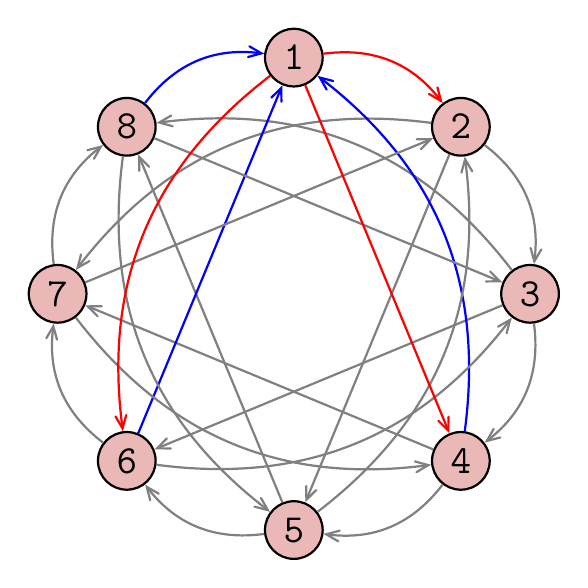
\begin{tikzpicture}[->,>=angle 45,shorten >=0pt,auto,node distance=2cm,
  thick,main node/.style={circle,fill=mymark,draw,font=\ttfamily\Large}]


  
  \foreach \a [count=\c] in {4,5,6,7,8,1,2,3}{
  \node[main node] (\a) at (\c*-360/8: 3cm) {\a};
}


  \path[every node/.style={font=\sffamily\small}]
(2)	edge [draw=black!50,bend left] node [] {} (3)
	edge [draw=black!50] node [] {} (5)
	edge [draw=black!50,bend right] node [] {} (7)
(3)	edge [draw=black!50,bend left] node [] {} (4)
	edge [draw=black!50] node [] {} (6)
	edge [draw=black!50,bend right] node [] {} (8)
(4)	edge [draw=black!50,bend left] node [] {} (5)
	edge [draw=black!50] node [] {} (7)
	edge [draw=blue,bend right] node [] {} (1)
(5)	edge [draw=black!50,bend left] node [] {} (6)
	edge [draw=black!50] node [] {} (8)
	edge [draw=black!50,bend right] node [] {} (2)
(6)	edge [draw=black!50,bend left] node [] {} (7)
	edge [draw=blue] node [] {} (1)
	edge [draw=black!50,bend right] node [] {} (3)
(7)	edge [draw=black!50,bend left] node [] {} (8)
	edge [draw=black!50] node [] {} (2)
	edge [draw=black!50,bend right] node [] {} (4)
(8)	edge [draw=blue,bend left] node [] {} (1)
	edge [draw=black!50] node [] {} (3)
	edge [draw=black!50,bend right] node [] {} (5)
(1)	edge [draw=red,bend left] node [] {} (2)
	edge [draw=red] node [] {} (4)
	edge [draw=red,bend right] node [] {} (6)

;
\end{tikzpicture}
\caption{De overdracht tussen 8 processen met een buffergrootte van 3. Uitgaande individuen van 1 zijn in het rood aangeduid. Binnenkomende individuen zijn in het blauw aangeduid.}
\label{parr_conn_8}
\end{figure}

\subsection{Minder processen dan aantal te versturen}
Als er minder procesen zijn dan te verzenden individu's dan zullen alle processen van alle andere processen minstens 1 individu krijgen. We sturen \[
\#(\text{per proces}) = \left\lfloor \frac{b}{p-1} \right\rfloor
\] individuen door naar elk ander proces.
Figuur~\ref{parr_conn_5} toont hoe de communicatie verloopt bij 5 processen en een buffergrootte van 8. We zien dat elk proces 2 individuen krijgt.
\begin{figure}[H]
\centering
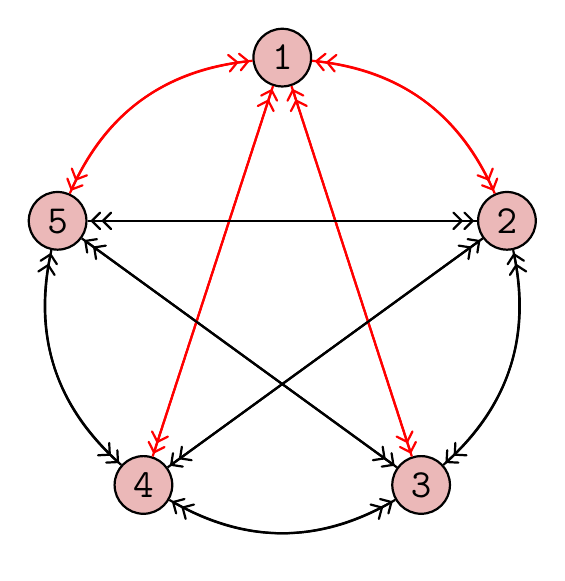
\begin{tikzpicture}[->>,>=angle 90,shorten >=1pt,auto,node distance=2cm,
  thick,main node/.style={circle,fill=mymark,draw,font=\ttfamily\Large}]

\foreach \a [count=\c]in {1,2,...,5}{
  \node[main node] (\a) at (162+\c*-360/5: 3cm) {\a};
}



  \path[every node/.style={font=\sffamily\small}]

(1)	edge [draw=red,bend left] node [] {} (2)
	edge [draw=red] node [] {} (3)
	edge [draw=red] node [] {} (4)
	edge [draw=red,bend right] node [] {} (5)
(2)	edge [bend left] node [] {} (3)
	edge node [] {} (4)
	edge node [] {} (5)
	edge [bend right,draw=red] node [] {} (1)
(3)	edge [bend left] node [] {} (4)
	edge node [] {} (5)
	edge [draw=red] node [] {} (1)
	edge [bend right] node [] {} (2)
(4)	edge [bend left] node [] {} (5)
	edge [draw=red] node [] {} (1)
	edge node [] {} (2)
	edge [bend right] node [] {} (3)
(5)	edge [bend left, draw=red] node [] {} (1)
	edge node [] {} (2)
	edge node [] {} (3)
	edge [bend right] node [] {} (4)




;
\end{tikzpicture}
\caption{De overdracht tussen 5 processen met 8 te versturen individuen. Uitgaande en binnenkomende individuen van 1 zijn in het rood aangeduid.}
\label{parr_conn_5}
\end{figure}

\section{Kopiëren of verplaatsen}
\label{sub:toCopyOrNotToCopy}
Elk process krigt nu evenveel individuen binnen als hij verstuurd. Wij kunnen nu 2 dingen doen:
\begin{enumerate}
	\item De verstuurde individuen overschrijven met de nieuwe individuen.
	\item De ontvangen individuen gewoon toevoegen aan de populatie en dan de populatie terug naar zijn oorspronkelijke grootte brengen zoals beschreven in sectie~\ref{sub:tournament}.
\end{enumerate}

Figuur~\ref{graf:nocopycopy} toont ons dat kopiëren nefast is voor de performantie.
We kunnen dit verklaren door op te merken dat bij het kopiëren de populatie als het ware veel duplicaten zal bevatten van verstuurde individuen. Dit zorgt er voor dat de ,genetische diversiteit afneemt. Wat op zijn beurt de daling in prestatie verklaart.

\begin{figure}[H]
\rnxaxisr{Fitness}{processors}{
	\addplotf{NUM_PROCESSORS_NOCOPY};
	\addplotf{NUM_PROCESSORS_COPY};
}

\nxaxisr{Tijd (s)}{processors}{
	\addplott{NUM_PROCESSORS_NOCOPY};
	\addplott{NUM_PROCESSORS_COPY};
}
\caption{Uitvoeringstijd en fitheid in functie van het aantal processoren voor het plaatsen van 500 punten in \texttt{vierkant.poly} met (geel) en zonder (groen) kopiëren}
\label{graf:nocopycopy}
\end{figure}

\section{Complexiteit}
\label{sub:parrcomplex}
We bepalen nu de complexiteit van het algoritme rekening houdend met het aantal processoren $p$.


Als we kijken naar de graieken uit \ref{graf:numIndividus} zien we dat zien we dat het aantal nodige iteraties exponentieel afneemt met stijgende populatiegrootte en dan stabliseert. We merken op dat de sterke stijging in uitvoeringstijd er net toe doet daar we het parallel uitvoeren met kleine populaties. Hoe meer processoren, hoe minder tijd er nodig zal zijn om te convergeren tot op het moment van stabilisatie. We kunnen schrijven dat, tot er stabilisatie is, het aantal iteraties $\Theta\left(\frac{n}{\log{p}}\right)$ is.

Daar we telkens even veel individuen versturen om kunnen we er van uitgaan dat het aantal het aantal uitwisselingen lineair is in het aantal te verzenden punten\footnote{wat evenredig is met $n$, het aantal te plaatsen punten}. We bekomen dus een complexiteit van $T(n)=\Theta\left(\frac{p\cdot n}{\log{p}}\right)$ voor de communicatie. 

%cat coppy | sed  "/^\s*$/{N;N;x;N;N;x;N;N;N;s/\n/,/g;s/^,//}; s/[^0-9.,]//g" | awk 'BEGIN{FS=",";OFS=",";print "testValue","f","t","usrt","syst";} $3 {print $2,$1,$3,$4,$5}' | sort -n

Zoals besproken in sectie~\ref{ssub:genetic} heeft het genetisch algoritme zelf een complexiteit van $T(n)=\Theta(n^2)$ per iteratie. 

Zolang de winst door het vergroten van de populatiegrootte niet stagneert is de complexiteit  \[T(n)=\Theta\left(\frac{p\cdot n + n^2}{\log{p}}\right) = \Theta\left(\frac{p\cdot n + n^3}{\log{p}}\right)\]. Nadat de winst door populatievergroting stagneert, wordt de noemer gewoon een constante. In figuur~\ref{delcaty} kan je dit fenomeen zien in de groene grafiek. Deze grafiek is geproduceerd door te weinig communicatie te voeren tussen processen waardoor de winst door populatievergroting verkleint. Bij ongeveer 24 processoren wordt de overhead door communicatie ($\Theta(p\cdot n)$) groter dan de winst door populatievergroting.

\section{Uitvoeren op HPC}
Om onze gedistribueerde code te testen maken we gebruik van de Pokémon\footnote{Dat is dus een supercomputer van het HPC} Delcatty. In figuur \ref{delcaty} zien we op de oranje grafiek bij het vergoten van het aantal processoren de fitheid stijgt en de uitvoeringstijd daalt. We merken echter op dat het dalen verbeteren initieel sterk is en daarna stagneert dit komt omdat er geen winst meer gehaald wordt uit het vergroten van de totale populatie. De groene graffiek geeft aan wat er gebeurt als er te men te veel tijd laat tussen synchronisaties (500 iteraties van het gewone algoritme in plaats van 50). Als we niet vaak genoeg synchroniseren emuleren we geen grotere populatie waardoor de winst door grotere populatie sterk wordt verminderd. We zien ook dat het eens de communicatie de overhand neemt de grafiek linear stijgt zoals uitgelerd in sectie \ref{sub:parrcomplex}.

\begin{figure}[H]

\rnxaxisr{Fitness}{processors}{
	\addplotf{NUM_PROCESSORS_BIG};
	\addplotf{NUM_PROCESSORS_NOCOPY};
}

\nxaxisr{Tijd (s)}{processors}{
	\addplott{NUM_PROCESSORS_BIG};
	\addplott{NUM_PROCESSORS_NOCOPY};
}
\caption{Uitvoeringstijd en fitheid in functie van het aantal processoren voor het plaatsen van 500 punten in \texttt{vierkant.poly} bij goed gekozen communicatiehoeveelheid (oranje) en te weinig communicatie (groen)}
\label{delcaty}
\end{figure}

\section{Vergelijking serieel}

\begin{figure}[H]
\rnxaxis{Fitness}{Aantal punten}{
	\addplotf{SEQ_MPI};
	\addplotf{SEQ_NOMPI};
}

\nxaxis{Tijd (s)}{Aantal punten}{
	\addplott{SEQ_MPI};
	\addplott{SEQ_NOMPI};
}
\caption{Uitvoeringstijd en fitheid in functie van het aantal te plaatsen punten in \texttt{vierkant.poly} serieel (oranje) en parallel (groen)}
\label{graf:perf}
\end{figure}

Figuur \ref{graf:perf} toont ons dat het gedistridueerde algoritme sneller is dan het serieel algoritme voor een groter aantal punten. Als er wijnig punten te plaatsen zijn zorgt de communicatie voor te veel overhead. In de data die tot de grafiieken leid zien we ook dat het parallel algoritme ook over het algemeen een fitheid geeft die net iets hoger ($< 0.1\%$) is dan bij serieel.


\section{Implementatie}
We bespreken nog hoe we de distributie hebben geïmplementeerd met MPI. Allereerst hebben we een functie gemaakt die het serieel algoritme voor een bepaald aantal iteraties uitvoert. Eens dit gedaan is, wordt een function pointer oproepen met pointer de huidge populatie en het aantal uitvoerde iteraties. Als deze oproep \texttt{GENETIC\_CONTINUE} teruggeeft, dan wordt er verder gegaan met itereren anders wordt er gestopt. De functie waar de functionpointer naar wijst is verschillend voor het master proces en de slave processen. 

Het master proces ontvangt telkens de fitheid van het beste individu en het percentage van het aantal gevraagde iteraties dat is uitvoert voor de stopvoorwaarde van het serieel algoritme werd bereikt\footnote{Als deze niet berei werd, word 100\% doorgestuurd} van de slaves met een \texttt{Gather}. Uit deze informatie leid het master proces af of er al dan niet gestopt moet worden. Als dat zo is stuurt hij een bericht naar alle slaves met \texttt{Send}. In dit bericht wordt het processID van het beste proces geplaatst. Het beste proces stuurt zijn beste individu terug naar de master die ze dan afbeeld op het scherm. Om zinloos wachten te vermijden doet het master proces, net als de slaves, ook iteraties van het genetisch algoritme.

De slave processen sturen de gegevens gevraagd door de master en stopen met itereren als de master dit vraagt. Er wordt gecontroleerd of de master een bericht heeft gestuurd met \texttt{IProbe}. Als het master proces een stop signaal geeft wordt \texttt{GENETIC\_BEST} of \texttt{GENETIC\_NOT\_BEST} teruggegeven waardoor het itereren zal stoppen. Anders wordt er \texttt{GENETIC\_CONTINUE} teruggegeven.

Om individuen door te sturen hebben we ze geserialiseerd tot een array van \texttt{float}s. 

% section  (end)

%\section{Bronnen}
Er moet vermeld worden dat het icosagon bestand afkomstig is van Jonathan Peck. 

\end{document}